\documentclass{article}
% Submission version: anonymous, line numbers, 8 pages main text.
% Compile with: tectonic main.tex   (bibliography: corlabbrvnat.bst, natbib numbers)
\usepackage{corl_2026}
\usepackage{graphicx}
\usepackage{booktabs}
\usepackage{xcolor}
\usepackage{amsmath,amssymb}
\usepackage{multirow}
\usepackage{microtype}
\usepackage{fontspec}
\setmainfont{texgyretermes}[Extension=.otf,UprightFont=*-regular,BoldFont=*-bold,ItalicFont=*-italic,BoldItalicFont=*-bolditalic]
\setsansfont{texgyreheros}[Extension=.otf,UprightFont=*-regular,BoldFont=*-bold,ItalicFont=*-italic,BoldItalicFont=*-bolditalic]
\newcommand{\todo}[1]{\textcolor{red}{[#1]}}
\newcommand{\sys}[1]{\textsc{#1}}

\title{Blame the Bowl, Not the Goldfish: Robot Memory\\Interference Is a Budget-Allocation Problem}

% Submission is double-blind: \anonfalse only for the camera-ready / arXiv version.
\newif\ifanon \anontrue
\ifanon
\author{Anonymous Author(s)\\Anonymous Institution\\\texttt{anonymous@example.org}}
\else
\author{Han Lee\\Stanford University\\\texttt{hanl@stanford.edu}}
\fi

\begin{document}
\maketitle

\keywords{memory, vision-language-action models, long-horizon manipulation, interference}

\begin{abstract}
Released memory-augmented $\pi_{0.5}$ policies lose most of their success when the demonstration they need is buried under $k$ unrelated sessions. We show that the policy has not forgotten how to act: it is handed the wrong frames. The 32-frame memory budget is filled by even sampling over a growing buffer, so the lesson's share of the budget shrinks with $k$; giving the same frozen policy the same 32 slots filled from the lesson session restores the no-interference success on every task we test, out to $k{=}15$, on two architectures. Interference in these policies is a \emph{budget-allocation} failure, and we frame memory as a decision question: a memory is worth exactly what it changes in the policy's action. A retrofitted manager must respect two things the frozen policy learned implicitly and recall-style metrics cannot see, the sampling comb of its own episode and the absolute-time positions of its frames; re-indexing positions recovers up to 28 points at $k{=}15$. Because RoboMME records the lesson in the scene the robot then acts in, the lesson is always the most similar session; we add a condition in which three distractors are recorded in the query scene itself, where similarity routing fails on three of four tasks ($.22$ vs $.70$ with oracle routing on RouteStick) and a label-free router that gates by scene and picks by the task \emph{instruction} in an off-the-shelf image--text space recovers the oracle where the lesson's content is visible in a frame, replicating on two further scene sets. Two negative results close the loop: training a manager on the policy's demonstration loss makes it discard the lesson, and fine-tuning the policy itself on the interference distribution flattens its curve only by lowering the no-interference ceiling, while fine-tuning on displaced positions moves it toward tolerating them without reaching significance. A mechanism study with an information-matched student in a grid world shows the same allocation effect with learned writers and isolates why a two-scale memory is needed to act on a hindsight-selected store.
\end{abstract}

% ------------------------------------------------------------------------------------------------
\section{Introduction}
\label{sec:intro}

Long-horizon manipulation increasingly relies on policies that look back over minutes, and across sessions, through a memory with a fixed token budget. MEM~\cite{mem} made the two-scale design concrete: a working memory of recent observations and a consolidated long-term store, with a hand-written compression policy deciding what enters the store. RoboMME~\cite{robomme} made the evaluation concrete, with a taxonomy of memory-dependent manipulation tasks and a suite of memory-augmented $\pi_{0.5}$ policies~\cite{pi05}, and RoboMME-Interference~\cite{robomme_interference} added the protocol in which the relevant lesson is buried under $k$ unrelated sessions. Both leave open the question this paper is about: \emph{what should a budgeted memory keep, and how should a manager decide?}

\begin{figure}[tb]
\centering
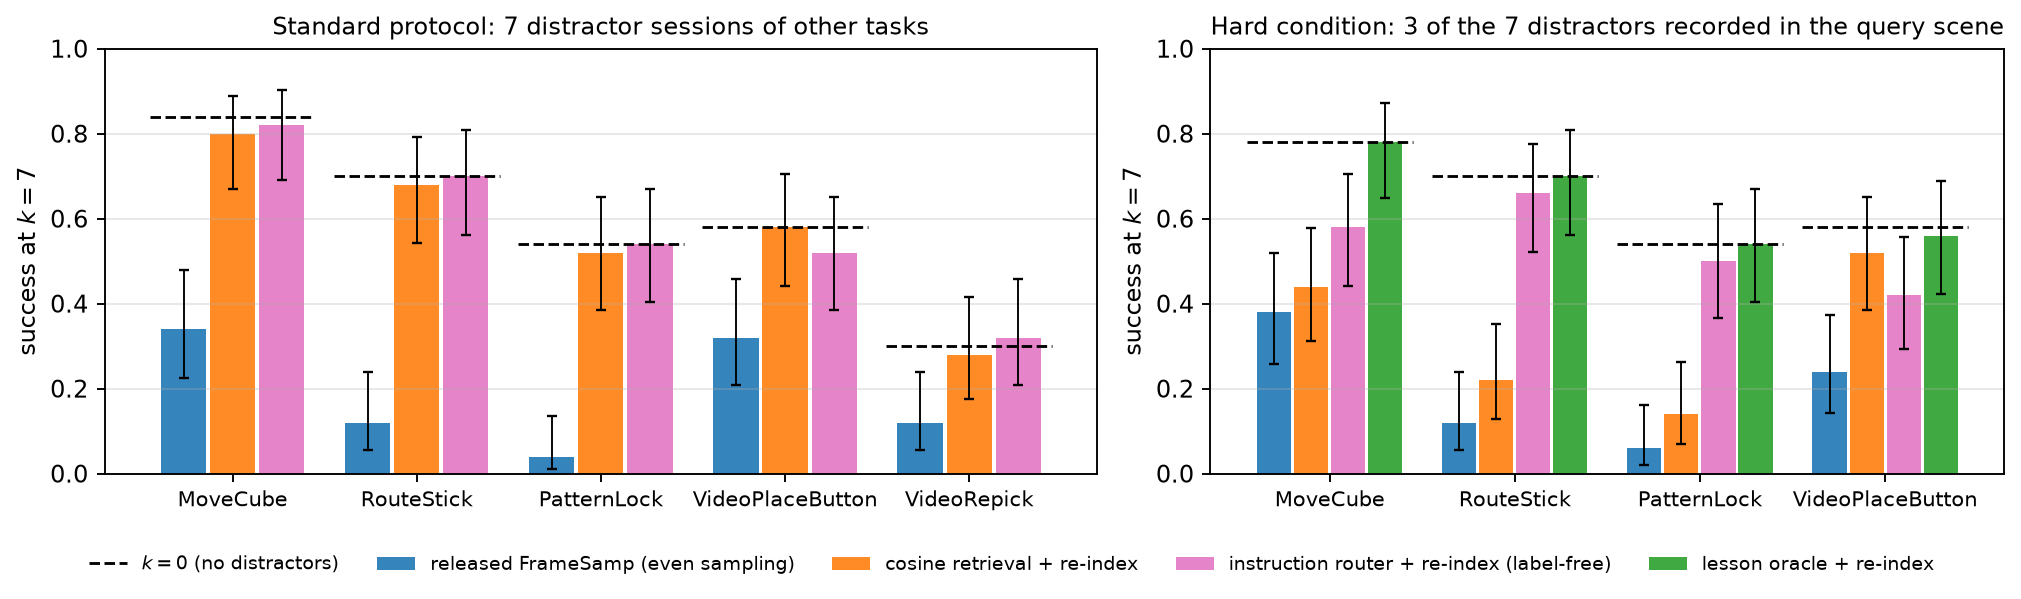
\includegraphics[width=\linewidth]{fig/headline.png}
\caption{The policy has the skill; the sampler spends the budget on the wrong frames. Success at $k{=}7$ distractor sessions for the released $\pi_{0.5}$ FrameSamp policy and for the same frozen policy with its 32 memory slots filled from the lesson session by three managers ($n{=}50$ per cell, Wilson 95\% intervals; dashed: the $k{=}0$ level). Left: the standard RoboMME-Interference protocol. Right: our hard condition, three of the seven distractors recorded in the query scene; cosine retrieval routes to the replays on three of four tasks.}
\label{fig:headline}
\end{figure}

The question looks like a compression question and is usually treated as one: keep what is salient, recent, or reconstructs the past well. We argue it is a decision question, and that the policies in question are not goldfish: they have not forgotten the lesson; the bowl, the sampler that fills their slots, hands them the wrong frames. A memory is worth exactly what it changes in the policy's action; anything the policy would do the same without it is waste at the budget, and anything that makes the policy act worse is harm. The paper tests four consequences. (i)~\textbf{Interference in a released memory VLA is a budget-allocation failure} (\S\ref{sec:budget}--\ref{sec:general}, Figure~\ref{fig:headline}): even sampling over a growing buffer dilutes the lesson's share of the 32 slots, and routing the budget to the lesson session removes the loss. The benchmark paper reports that a scene-split retrieval step in front of the same policy is flat in $k$~\cite{robomme_interference}; we confirm that, explain it through the lesson oracle and the lesson's budget share, and show that a retrofitted manager must also respect two things the frozen policy learned implicitly (\S\ref{sec:constraints}): the sampling comb of its own episode and the absolute-time positions of its frames, whose shift alone costs up to 28 points at $k{=}15$. (ii)~\textbf{Hard routing} (\S\ref{sec:hard}): because RoboMME's lesson is recorded in the scene the robot then acts in, it is always the most similar session. Real deployments are not like that: the robot has usually been in this scene before, doing other things. When three distractor sessions are replays of unrelated motions \emph{recorded in the query scene}, similarity routing fails on three of four tasks, the budget fix under oracle routing still holds in full, and a label-free router that gates sessions by scene and chooses by the task \emph{instruction} in an off-the-shelf image--text space, with no training, recovers the oracle where the lesson's content is visible in a frame. (iii)~\textbf{Training is not a substitute for allocation} (\S\ref{sec:train}): fine-tuning the policy on the interference distribution it is evaluated on removes most of its loss there and none of its interference; it flattens the success curve by lowering the no-interference ceiling. Fine-tuning on displaced positions moves the policy toward tolerating them, consistently across two splits but short of significance. (iv)~\textbf{The hindsight gap} (\S\ref{sec:pantry}): in a grid world with learned writers, deciding at write time behaves like recency under interference; deciding at session boundaries closes the gap, but only beside a working memory.

We also report what did not work (\S\ref{sec:negative}). Scoring memories by the frozen policy's own demonstration loss learned the loss landscape faithfully and discarded the lesson, because under interference the loss on expert demonstrations is lower with recent frames than with the lesson. The decision value of a memory is a closed-loop quantity.

\paragraph{Contributions.} (1)~A diagnosis of cross-session interference in released memory VLAs as a budget-allocation failure, two retrofit constraints invisible to recall metrics (one a positional-shift mechanism new to memory VLAs), and a label-free fix that holds across five tasks, two splits and two architectures. (2)~A hard-routing condition for RoboMME-Interference in which the lesson is no longer the most similar session, on four tasks and three scene sets, with label-trained and label-free instruction-conditioned routers that recover the oracle level. (3)~A controlled fine-tuning study showing that training the policy on the interference distribution does not repair the allocation and damages the no-interference case, with a faithful control. (4)~Two negative results with their mechanisms, and a decision-sufficiency account of budgeted memory with a grid-world mechanism study of learned writers.

% ------------------------------------------------------------------------------------------------
\section{Related work}
\label{sec:related}

\textbf{Memory for VLAs.} MEM~\cite{mem} organises memory at two scales and compresses the long-term store with an LLM prompt; MemER~\cite{memer} keeps key frames selected by a VLM; DeMem~\cite{demem} argues for decision-aware memory for language agents. RoboMME's model suite~\cite{robomme} spans symbolic, perceptual (frame sampling, token dropping) and recurrent (RMT~\cite{rmt}, TTT~\cite{ttt}) representations, integrated as context, modulation or a separate memory expert; the released frame-sampling models are the subject of \S\ref{sec:scale}, and RoboMME-Interference~\cite{robomme_interference} supplies the cross-session protocol we adopt unchanged and the retrieval baseline we build on and then break. We hold the architecture fixed and ask what the budget should hold.

\textbf{Positions and forgetting.} Length-generalisation failures of absolute and rotary positions are documented for language models~\cite{alibi,lengthgen}; the variant we find, a shift of the current episode's positions relative to the retrieved session, is specific to buffers that grow with sessions and has to our knowledge not been reported for robot policies. Predictive forgetting and test-time memorisation~\cite{titans} decide what to keep from signals computed at write time; our results say \emph{when} the decision is made and \emph{which signal} drives it matter more than how it is made.

% ------------------------------------------------------------------------------------------------
\section{Decision-sufficient memory}
\label{sec:theory}

Let $\pi$ act on the current observation $o$ and a memory $m$ of budget $B$, and let $\pi^\star$ be the same policy with the full history $h$. The \textbf{decision distortion} $D(m)=\mathbb{E}\,\|\pi(o,m)-\pi^\star(o,h)\|$ measures what the memory changes in the action: a memory is good iff $D(m)$ is small, and any objective not monotone in $D$ (reconstruction, coverage, recency, similarity) can be made arbitrarily bad at the same budget. Two counting consequences drive the experiments (statements and proofs in Appendix~\ref{app:theory}): a \textbf{hindsight gap}, by which a writer deciding at write time retains fewer still-valid facts than one deciding at session end, and an \textbf{interference collapse}, by which any decision-blind allocation (recency, FIFO, even sampling) gives the relevant session a budget share that falls as $1/(1+km/D)$ with $k$ distractor sessions of $m$ units against a lesson of $D$, while a decision-aware allocation is flat in $k$. We isolate the schedule effect where the decision has a ground truth (\S\ref{sec:pantry}), then test the allocation prediction on released policies (\S\ref{sec:scale}).

% ------------------------------------------------------------------------------------------------
\section{Pantry: a mechanism study with an information-matched student}
\label{sec:pantry}

Pantry exists for one thing RoboMME cannot give: a ground-truth decision and writers that can be \emph{learned}, so the write schedule can be isolated from everything else. Its result motivates the two-scale layout that \S\ref{sec:scale} takes as given.

\textbf{Setup.} Pantry is a $9{\times}9$ grid world ($64{\times}64$ RGB) with auto-closing drawers, an opaque bin, a cue panel that blanks after three steps, buttons, and a cabinet whose hidden latch jams after a wrong strategy. Tasks follow the RoboMME taxonomy (\emph{find}, \emph{count}, \emph{sequence}, \emph{adapt}, \emph{tidy}) and trials follow RoboMME-Interference: session~0 reveals facts about layout $L_0$, then $k\in\{0,1,3,7\}$ distractor sessions on other layouts, then a query on $L_0$ solvable only from memory. A belief-state expert acts on the events it has observed, so ``what to remember'' has a ground truth, and an information-matched student (2.2M-parameter transformer over four frames, context tokens and $B$ memory slots) imitates the expert's action computed from \emph{exactly} the information the student is given (98.9\% per-step agreement; 97--100\% success with oracle memory). Memory units are typed event facts or frames, mirroring MEM's text and video tracks.

\textbf{Memory systems.} Recency, reservoir random, a scripted MEM-style compressor (latest fact per drawer, drop superseded facts and failed strategies, FIFO at the budget), an oracle that protects the facts the future query needs, and four writers trained with GRPO~\cite{grpo} against the frozen student, rewarded by the student's log-probability of the full-information expert's action on memory-relevant steps: \emph{online} (at each event, overwrite a slot or drop), \emph{hindsight consolidator} (re-select $B$ items at session end without seeing the next task), \emph{both}, and \emph{two-scale} ($B/2$ online slots cleared at session end plus $B/2$ consolidated slots).


\textbf{Results} (Table~\ref{tab:pantry}, Appendix~\ref{app:pantry}; $B{=}8$, 90 trials per $k$). At $k=0/1/3/7$: recency $.94/.36/.00/.00$, scripted compressor $.99/.99/.76/.22$, learned online writer $.98/.76/.42/.27$, hindsight consolidator $.29/.31/.12/.13$, learned two-scale $.96/.86/.79/.71$, oracle $.94/.87/.79/1.0$. (i)~The interference step of \S\ref{sec:theory} appears exactly: recency is at the no-memory level from $k{=}1$ and the scripted compressor decays from the oracle level to 22\%. (ii)~The learned online writer collapses like recency ($B{=}4$: $.80\to.03$ by $k{=}3$): the write schedule, not the learning, is the limit. (iii)~The hindsight consolidator is the best \emph{selector} (decision distortion $.78$ at $k{=}7$ against $.50$ for the compressor) and the worst closed-loop system: without a working memory the student cannot execute session~0, so the facts it would later need are never generated; the two-scale design fixes exactly this. The learned consolidator also keeps failed strategies (9\% of slots) that MEM's ``drop failures'' rule discards; that rule costs 25 points on adaptation. Budgets $B{=}2,4$ and the distortion tables are in Appendix~\ref{app:pantry}.

% ------------------------------------------------------------------------------------------------
\section{Scale: released memory VLAs on RoboMME-Interference}
\label{sec:scale}

\subsection{Protocol, model and systems}
\label{sec:protocol}

We use the released $\pi_{0.5}$ FrameSamp-Modul checkpoint of RoboMME~\cite{robomme} (and FrameSamp-Expert in \S\ref{sec:general}): a budget of 512 tokens $=$ 32 front-camera frames $\times$ 16 tokens, sampled evenly over the whole buffer at every call, with positional embeddings indexed by absolute step. RoboMME-Interference builds the buffer as [lesson video][$k$ distractor sessions][current episode], a distractor being a 32-frame unit from a recorded episode of another task family. We serve the released checkpoint unchanged and replace only the function that chooses the 32 frames: a \emph{memory manager} on the policy server that sees the buffer's SigLIP features~\cite{siglip} and the session boundaries and returns 32 indices (and, for re-indexing, their positions). Every system sees the same policy, scenes and distractors (common seeds). Test split, 50 episodes per cell (the split's full size), Wilson intervals; because every system runs on the same episodes, systems are compared with exact paired McNemar tests on the discordant episodes (Fisher exact tests only across splits); our released-baseline reproduction matches the published VideoRepick curve. All nine lesson tasks read ``watch the video carefully, then \ldots''; of the seven the released policy can perform, five are interference-sensitive and are used here (VideoPlaceOrder is flat in $k$).

\textbf{Systems.} \sys{released}: even sampling. \sys{recency}: the last 32 frames. \sys{two-scale}: the 16 most recent frames plus the lesson sampled evenly (MEM-style). \sys{lesson oracle}: the lesson session plus the current episode, session given. \sys{retrieval}: the session most cosine-similar (pooled SigLIP, max over frames) to the current view, plus the current episode. \sys{+~re-index}: the same frames with positions compacted to the trained layout. \sys{learned}: a selector trained by GRPO on the policy's demonstration loss (\S\ref{sec:negative}). Structured systems change only the history slots; the current episode keeps its even-sampling frames.

\begin{figure}[tb]
\centering
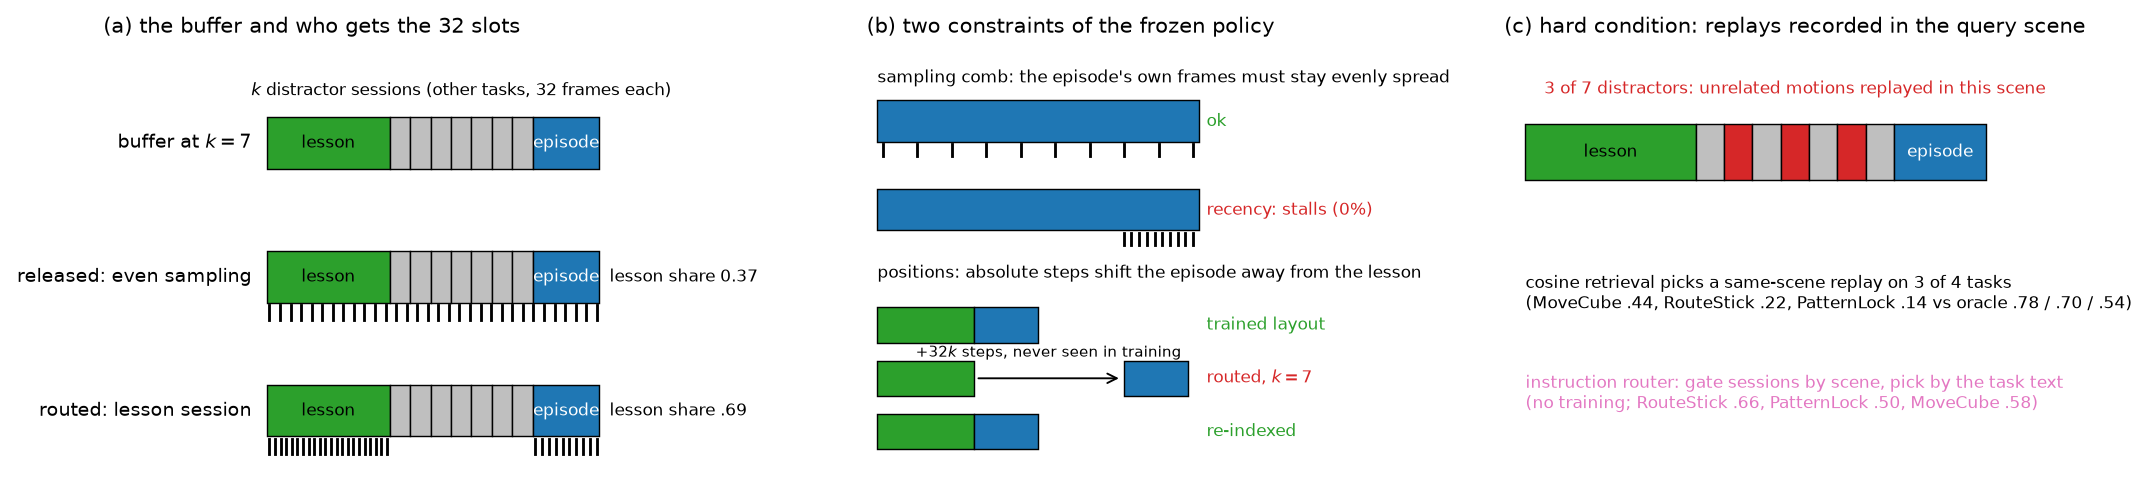
\includegraphics[width=\linewidth]{fig/schematic.png}
\caption{(a)~The buffer and the two allocations compared throughout: even sampling lets the lesson's share of the 32 slots fall with $k$; routing the slots to the lesson session holds it. (b)~The two constraints on a frozen policy: the current episode keeps its even comb, and positions are re-indexed to the trained layout. (c)~The hard condition: three distractors are unrelated motions replayed in the query scene.}
\label{fig:schematic}
\end{figure}

\subsection{Interference is a budget-allocation failure, and routing is trivial here}
\label{sec:budget}

\textbf{Takeaway: the released policy loses to interference because even sampling halves the lesson's share of its slots; give the slots to the lesson and the loss is gone.} 
The released model's interference is real (Table~\ref{tab:budget}, Appendix~\ref{app:dev}: VideoRepick $.30/.20/.12$ and VideoPlaceButton $.58/.46/.32$ at $k=0/3/7$, $p=.012$ and $.002$; $.52/.54/.28$ against same-task distractors, $p=.004$), and the lesson's share of the 32 slots falls from $.78$--$.89$ at $k{=}0$ to $.48$--$.70$ at $k{=}7$ under even sampling. Giving the budget to the lesson session holds the share at $.87$--$.89$ and removes the loss on VideoPlaceButton ($+.24$ at $k{=}7$, $p=.008$; $+.30$ against same-task distractors, $p=3\times10^{-4}$); VideoRepick has a low ceiling with this checkpoint and its gain becomes significant with re-indexing. Cosine similarity picks the lesson in 99--100\% of held-out draws. The reason is structural: in RoboMME the lesson is recorded in the scene instance the robot then acts in, so it is the most similar session \emph{by construction}; this is why the benchmark paper's own retrieval step is flat in $k$~\cite{robomme_interference}. The released model fails only because even sampling dilutes the budget; \S\ref{sec:hard} removes the benchmark's property by construction.

\subsection{Two constraints on a retrofitted manager}
\label{sec:constraints}

\textbf{Takeaway: a manager may change which history frames fill the slots, but not how the current episode is sampled or where in time the frames appear to sit.} \textbf{The sampling comb.} The frozen policy works only when its own episode is presented with the comb it was trained with: recency scores 0 on VideoRepick even at $k{=}0$ and runs ${\sim}950$ steps per episode instead of ${\sim}180$ (the policy stalls), and a MEM-style dense recent window scores $.02$--$.04$. A manager may only touch the long-term slots.

\textbf{Positional re-indexing.} Each memory frame carries a positional embedding of its absolute step. Under oracle routing at $k$ the \emph{frames} are the $k{=}0$ frames, but the current episode's positions are shifted by $32k$ steps away from the lesson, a layout never seen in training. Compacting the selected frames' positions to the trained layout (the lesson keeps $0..D{-}1$, the current episode continues from $D$) holds the oracle at the $k{=}0$ level on VideoRepick ($.32/.32$ vs $.28/.20$ at $k=3/7$; $p=.03$ at $k{=}7$) and makes retrieval + re-index flat in $k$ on both tasks (VideoRepick $.28/.28$ vs released $.20/.12$, $p=.02$; VideoPlaceButton $.58/.58$ vs $.46/.32$, $p=.004$). A shift-only ablation isolates the mechanism: the $k{=}0$ frames with the episode's positions moved by 96 or 224 steps and \emph{no distractor frames} score $.24$ and $.18$ on VideoRepick (from $.30$) and $.52$ on VideoPlaceButton. At $k{=}15$ the released model is at $.00$ and $.28$ while retrieval + re-index stays at $.32$ and $.56$ ($p=3\times10^{-5}$ and $.003$); the VideoPlaceButton result replicates on the val split ($.28$ vs $.60$ at $k{=}7$, $p=9\times10^{-4}$; pooled $n{=}100$: $.30$ vs $.59$, $p=5\times10^{-6}$).

\subsection{Generality: three more tasks, a second architecture, one label-free system}
\label{sec:general}


\begin{figure}[tb]
\centering
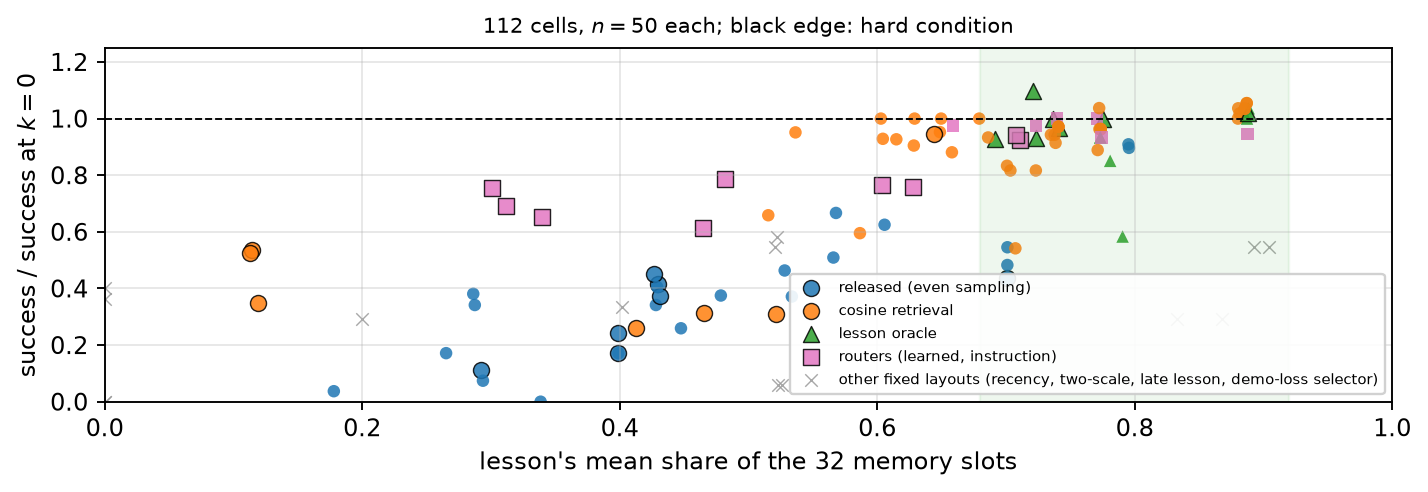
\includegraphics[width=.9\linewidth]{fig/mechanism.png}
\caption{Every evaluated cell of \S\ref{sec:scale} ($n{=}50$ each): success relative to the task's $k{=}0$ level against the lesson's mean share of the 32 slots. Success tracks the share; the band marks the share even sampling gives the lesson at $k{=}0$. Points with a high share but low success are the layouts that break a constraint of \S\ref{sec:constraints}: the oracle without re-indexing (positional shift) and the dense-recent and late-lesson layouts (comb).}
\label{fig:mechanism}
\end{figure}

\textbf{Takeaway: the same diagnosis and the same fix hold on five tasks and two architectures, and the policy's success is a function of the lesson's slot share (Figure~\ref{fig:mechanism}).} On every task (Table~\ref{tab:general} and Figure~\ref{fig:k}, Appendix~\ref{app:hard}; MoveCube $.84/.56/.34/.32$, PatternLock $.54/.14/.04/.02$, RouteStick $.70/.26/.12/.12$ at $k=0/3/7/15$, interference $p\le4\times10^{-7}$) the released model loses most of its success by $k{=}7$ and the manager stays at the $k{=}0$ level at every $k$: no retrieval + re-index cell differs from its $k{=}0$ cell ($p\ge.6$). Re-indexing becomes individually significant here: on MoveCube at $k{=}15$, where the current episode sits 480 steps after the lesson, retrieval alone falls to $.50$ and $.54$ on the two checkpoints while re-indexing holds $.78$ on both ($p=5\times10^{-4}$, $.01$); on the short PatternLock and RouteStick episodes the shift costs nothing measurable. FrameSamp-Expert reproduces the collapse, the recovery and the size of the positional-shift loss with the manager code unchanged. Finally, the label-free \emph{instruction router} introduced for the hard condition in \S\ref{sec:hard}, run unchanged on the standard protocol (Figure~\ref{fig:headline}, left), is at the $k{=}0$ level on all five tasks (MoveCube $.82$, PatternLock $.54$, RouteStick $.70$, VideoPlaceButton $.52$, VideoRepick $.32$; $p\ge.38$ against each $k{=}0$ cell, $p\le.03$ against the released model on all five) and routes 248 of 250 decisions to the lesson: one system covers both conditions.

\subsection{Negative result: the policy's demonstration loss undervalues memory}
\label{sec:negative}

The natural way to learn a manager for a frozen policy is to use the policy's own loss as the reward. We trained the long-term frame selector with GRPO on the frozen policy's flow-matching loss on held-out oracle demonstrations. The selector learned the loss landscape faithfully and discarded the lesson under interference: its lesson share fell to $.23$ at $k{=}7$ and success to $.32/.12/.10$ at $k=0/3/7$ on VideoRepick, below the released model, because at $k{=}7$ the demonstration loss on expert trajectories is \emph{lower} with recent distractor frames in memory than with the lesson. Decision-relevant steps are sparse, and per-step imitation loss on expert trajectories does not see the closed-loop recovery value the lesson provides when the policy is off the expert's path. A learned manager at scale needs a closed-loop or counterfactual reward, not a demonstration loss.

\subsection{Hard routing: when the lesson is not the most similar session}
\label{sec:hard}


\textbf{Takeaway: with distractors recorded in the query scene, similarity routing collapses on three of four tasks while the budget fix under oracle routing holds in full; a label-free router that reads the task instruction recovers the oracle where the lesson's content is visible in a frame.} Because the lesson is recorded in the acting scene, RoboMME's distractors are always \emph{less} similar to the current view than the lesson. We add a condition in which $m$ of the $k$ distractor sessions are \emph{recorded in the query scene itself}: after the lesson video has played, the robot replays the post-demonstration joint trajectory of a recorded episode of another task in this scene for 256 steps, and the resulting 32-frame session (same objects, lighting and camera as the current view; unrelated motion; no lesson content) is inserted among the distractors at a random position; the scene is then reset for the query episode (Appendix~\ref{app:hard}). We use $k{=}7$, $m{=}3$, $n{=}50$ on MoveCube, RouteStick, PatternLock and VideoPlaceButton (Figure~\ref{fig:headline} right; per-system bars, routing counts and all paired tests in Appendix~\ref{app:hard}, Figure~\ref{fig:hard} and Table~\ref{tab:hardstats}).

\textbf{Similarity fails on three of four tasks; the budget fix survives on all.} MoveCube: released $.78\to.38$ ($p=10^{-5}$); cosine retrieval + re-index $.44$, routing to a same-scene session in 45 of 50 episodes ($p=.55$ vs released); lesson oracle + re-index $.78$, the $k{=}0$ level ($5\times10^{-4}$ vs cosine). RouteStick: released $.70\to.12$, cosine $.22$ (a replay outright in 16 episodes; on the rest it flickers between lesson and replays as the robot moves), oracle $.70$. PatternLock: released $.54\to.06$, cosine $.14$ (the budget split between lesson and replay in most episodes), oracle $.54$. VideoPlaceButton is the exception that locates the failure: released $.58\to.24$, oracle $.56$, and cosine $.52$ ($p=.003$ vs released, $.69$ vs oracle), because the lesson there is a demonstration video with a different appearance from the live scene and the same-scene replays take only $.18$ of its slots; where the lesson looks like the scene it was recorded in, similarity cannot tell it from a replay. The FrameSamp-Expert checkpoint on MoveCube gives the same picture (released $.34$, cosine $.44$, oracle $.90$; Appendix~\ref{app:hard}). The budget fix works in full; the routing that carried it on the standard protocol fails wherever the lesson is not visually set apart from the scene.

\textbf{Routing is learnable in-task; transfer is one-directional.} A session router trained with labels on the train split, with same-scene sessions of 50 training scenes as negatives, routes 47 of 50 MoveCube test episodes correctly and scores $.78$, the oracle level; on RouteStick it mis-routes none and scores $.68$ ($p=1.0$ vs oracle; $2\times10^{-7}$ vs cosine). The MoveCube-trained router applied to RouteStick scores $.18$, mis-routing 37 of 50: it learned what a MoveCube lesson looks like, not what the lesson for this scene is. Leave-one-task-out, a router trained on three other tasks routes all 50 RouteStick test episodes correctly ($.70$); the same construction fails on MoveCube ($.44$; $.54$ with six training tasks), where offline it identifies the right \emph{scene} perfectly but picks the lesson among three same-scene sessions only $.44$ of the time (chance $.25$). Scene identification transfers; telling a demonstration from a replay in the same sparse scene by appearance does not. The router has to be told what the lesson is \emph{about}.

\textbf{A label-free instruction-conditioned router.} The instruction names what the lesson is about, so we route by it. In the joint image--text space of an off-the-shelf SigLIP model (so400m), a session is a scene candidate if the best cosine between one of its frames and the current view is within a margin of the best session's; among candidates we take the session whose frames best match the instruction (the goal string without its preamble). One decision per episode, the chosen session re-indexed: no training, no labels, nothing task-specific; the gate margin, the one free parameter, is set to $.03$ by an offline sweep on the train split (Appendix~\ref{app:hard}). On RouteStick the router scores $.66$, the oracle level ($p=.62$ vs oracle; $10^{-7}$ vs released, $3\times10^{-6}$ vs cosine), routing 48 of 50 episodes to the lesson; on PatternLock $.50$ vs oracle $.54$ ($p=.62$; $3\times10^{-6}$ vs released, $3\times10^{-4}$ vs cosine), routing 46 of 50. In every episode the gate admits exactly the lesson and the same-scene replays, so the whole decision is the instruction match among them. On MoveCube it scores $.58$, above the released model ($p=.013$) and below the oracle ($p=.006$): it picks the lesson in 20 of 50 episodes and a replay in 26, and when it picks the lesson it succeeds 19 times in 20; on the FrameSamp-Expert checkpoint the same router scores $.60$ (released $.34$, $p=.007$; cosine $.44$, $p=.008$; oracle $.90$). A 7B vision--language model~\cite{qwen25vl} asked whether a filmstrip of the session performs the instruction gives the same split offline (Appendix~\ref{app:vlm}). The instruction closes the gap where the lesson's content is visible in a frame (a stick on a route, a drawn pattern) and not where it is a short motion in a sparse scene (a cube arriving at a target), which neither model reads reliably from a handful of 256-pixel frames.

\textbf{Replication on two further scene sets.} On the val split of RouteStick (50 new scene instances and same-scene recordings) the ordering holds: released $.14$, cosine $.18$ ($p=.79$ vs released), instruction router $.44$ ($p=7\times10^{-4}$ vs released, $.007$ vs cosine), oracle $.56$, $k{=}0$ $.58$; here the router sits below the oracle ($p=.03$, six discordant episodes, all in the oracle's favour) rather than at it. On the val split of MoveCube: released $.32$, cosine $.30$, instruction router $.56$ ($p=.008$ vs released), oracle $.80$, $k{=}0$ $.86$ ($p=.25$ vs oracle), the same ordering as the test split (Appendix~\ref{app:hard}). On VideoPlaceButton the router scores $.42$, between cosine and released ($p=.02$ vs released, $.04$ vs oracle): the instruction is nearly the same across that task's sessions, so the text match adds little where the scene gate already suffices. What remains on MoveCube is a perception limit, not a memory-management one: the manager knows what to look for and lacks a reader that can see it.

\subsection{Can training fix it at the source?}
\label{sec:train}

\begin{table}[tb]
\centering\small
\caption{Fine-tuning the released policy for 4000 steps on three training distributions, served with the \emph{unchanged} even-sampling memory ($n{=}50$, test split). \sys{control}: the released recipe. \sys{shift}: the current episode's positions displaced by $32k$ steps, the layout a retrieval manager produces. \sys{interf}: the interference buffer itself with even sampling, the layout the released sampler faces. Bold: differs from \sys{control} at $p<.05$ (paired McNemar).}
\label{tab:train}
\setlength{\tabcolsep}{5pt}\footnotesize
\begin{tabular}{llcccc}
\toprule
task & cell & released & \sys{control} & \sys{shift} & \sys{interf}\\
\midrule
MoveCube & even sampling, $k{=}0$ & .84 & .72 & .74 & \textbf{.52}\\
MoveCube & even sampling, $k{=}7$ & .34 & .30 & .32 & .30\\
MoveCube & retrieval, $k{=}15$ & .50 & .60 & .68 & \textbf{.38}\\
MoveCube & retrieval + re-index, $k{=}15$ & .78 & .66 & .72 & .54\\
RouteStick & even sampling, $k{=}0$ & .70 & .72 & .70 & \textbf{.40}\\
RouteStick & even sampling, $k{=}7$ & .12 & .14 & .14 & .22\\
VideoPlaceButton & even sampling, $k{=}0$ & .58 & .50 & .56 & .50\\
VideoPlaceButton & even sampling, $k{=}7$ & .32 & .22 & .20 & .38\\
\bottomrule
\end{tabular}
\end{table}

\textbf{Takeaway: fine-tuning the policy on the interference distribution removes most of its loss there and none of its interference; it lowers the no-interference ceiling instead.} Would the collapse and the constraints disappear if the policy were trained on the distribution it is evaluated on? Starting from the released checkpoint we fine-tune all non-vision parameters (2.9B, EMA $.99$, learning rate $10^{-5}$ with cosine decay, batch 32, 4000 steps on 500 episodes of five tasks, one H100 for 55 minutes per run; Appendix~\ref{app:train}) under three training distributions and serve every result with the released sampler (Table~\ref{tab:train}). \sys{control} is within noise of the released checkpoint on all nine cells, so the recipe is faithful. \sys{shift} moves the way the positional diagnosis predicts, but not far enough to call: plain retrieval at $k{=}15$, which re-indexing lifts from $.50$ to $.78$ on the released policy, reaches $.68$ on the test split and $.60$ on the val split (released $.54$, \sys{control} $.54$). Pooled ($n{=}100$) it has the highest plain-retrieval score ($.64$ vs $.57$ \sys{control}, $p=.19$; vs $.52$ released, $p=.04$) and the smallest re-indexing gap ($.10$, $p=.04$, vs $.13$ \sys{control} and $.24$ released; Appendix~\ref{app:train}): consistent with a trained-in habit, not a demonstration of one. Re-indexing at test time, which costs nothing, remains the established fix. \sys{interf} does not fix interference. At $k{=}7$ success is unchanged on MoveCube ($.30$) and within noise elsewhere, while the no-interference case drops (RouteStick $k{=}0$ $.72\to.40$, $p=4\times10^{-4}$; MoveCube $.72\to.52$, $p=.02$) and retrieval at $k{=}15$ gets worse ($.60\to.38$, $p=.013$). Its training loss fell from $.0060$ to $.0010$, so the policy did learn the distribution; what it learned was to lean less on memory, because no training recovers information the sampler never hands over (the lesson holds about 14 of the 32 slots at $k{=}7$ in training and at test alike). Fine-tuning on the interference distribution flattens the curve by lowering its ceiling; it is not a substitute for allocating the budget.

% ------------------------------------------------------------------------------------------------
\section{Discussion}
\label{sec:discussion}

\textbf{For MEM-style systems.} Organise the long-term store at the \emph{session} level and allocate the budget to the relevant session before any within-session compression; even sampling over a growing buffer is decision-blind and decays as \S\ref{sec:theory} predicts. Consolidate at session boundaries, with a working memory beside it, and condition routing on what the policy is asked to do, not only on what the scene looks like. Recall-style metrics would rate every structured system in \S\ref{sec:scale} identically, since all contain the lesson; the constraints, the routing failures and both negative results are only visible closed-loop. Absolute-time positions are a liability for growing buffers; re-indexing removes it at test time and training on displaced positions appears to reduce it (\S\ref{sec:train}). Training on the interference distribution does not remove the interference, because the allocation decision cannot be folded into the policy's weights while the sampler is fixed; and demonstration loss is not a usable reward for a manager. Together these point at the component this paper does not build: a learned, frame-level allocator trained from the policy's closed-loop behaviour, with the lesson oracle as its target and the hard condition as its test.

\textbf{Limitations.} $n=50$ per cell (the test split's size), partly offset by replication on the val split, five tasks and two checkpoints; all experiments are in simulation. The fine-tuning study uses one recipe and 4000 steps: it shows that this recipe does not repair the allocation, not that no training could, and the \sys{shift} effect is $+.07$ against \sys{control} at $n{=}100$ ($p=.19$). The hard condition is one construction, and cosine retrieval survives it on the one task whose lesson is visually set apart.

\clearpage
\acknowledgments{Removed for anonymous review.}

\bibliography{refs}

\clearpage
\appendix
\section{Statements and proofs for Section~\ref{sec:theory}}
\label{app:theory}

\textbf{Decision sufficiency.} Let $J(m)$ be the expected return of $\pi(\cdot,m)$ and $J^\star$ that of $\pi^\star(\cdot,h)$. For a policy whose return is $L$-Lipschitz in its action, $J^\star - J(m)\le L\,T\,D(m)$ over a horizon $T$, so a small decision distortion suffices. Conversely, for any objective $F(m)$ not monotone in $D$ there exist two memories $m_1,m_2$ at the same budget with $F(m_1)<F(m_2)$ and $D(m_1)>D(m_2)$; a history in which the decision-relevant content is a single unit unlike the bulk realises this for reconstruction, coverage, recency and similarity objectives at once, since each prefers the bulk. This transfers the argument of~\cite{demem} from bandits to sequential imitation.

\textbf{Hindsight gap.} A session emits $n$ facts in sequence; each is superseded later in the session independently with probability $s/n$ (so $s$ are superseded in expectation), and supersession is not predictable at emission. A causal writer with budget $B$ that keeps a fact at emission keeps a still-valid fact with probability $1-s/n$ regardless of its rule, so it holds at most $B(1-s/n)$ valid facts in expectation at session end. A consolidator that selects at session end sees which facts were superseded and keeps $\min(B,n-s)$ valid facts. The gap $\min(B,n-s)-B(1-s/n)$ is positive whenever $0<s<n$ and $B\le n-s$, and depends only on the write schedule.

\textbf{Interference collapse.} A decision-blind store draws its $B$ slots from the buffer with a rule that does not depend on the content's relevance: recency, FIFO, or even sampling. With $k$ distractor sessions of $m$ units and a lesson of $D$ units, even sampling gives the lesson a share $D/(D+km)$ of the slots, i.e. $B\,D/(D+km)=B/(1+km/D)$ slots; FIFO and recency give it $\max(0,B-km)$, which is smaller. If the policy needs at least $b^\star$ lesson slots to act (Pantry: one fact; RoboMME: a share above roughly $.7$, \S\ref{sec:budget}), success is a decreasing function of $k$ with a step at $k^\star=D(B/b^\star-1)/m$. A decision-aware allocation that gives the lesson $b^\star$ slots whenever it is present is flat in $k$.

\section{Pantry: additional results}
\label{app:pantry}

\begin{table}[h]
\centering\small
\caption{Pantry: closed-loop query success at budget $B{=}8$ against $k$ distractor sessions (90 cross-session trials per $k$). Only the two-scale learned memory and the oracle hold under interference.}
\label{tab:pantry}
\setlength{\tabcolsep}{5pt}
\begin{tabular}{lcccc}
\toprule
system & $k{=}0$ & $k{=}1$ & $k{=}3$ & $k{=}7$\\
\midrule
recency (facts) & .94 & .36 & .00 & .00\\
random & .94 & .67 & .34 & .22\\
scripted MEM-style compressor & .99 & .99 & .76 & .22\\
online writer (learned) & .98 & .76 & .42 & .27\\
hindsight consolidator (learned) & .29 & .31 & .12 & .13\\
two-scale (learned) & \textbf{.96} & \textbf{.86} & \textbf{.79} & \textbf{.71}\\
oracle & .94 & .87 & .79 & 1.0\\
\bottomrule
\end{tabular}
\end{table}

\begin{table}[h]
\centering\small
\caption{Pantry closed-loop query success by $k$ at budgets $B{=}2$ and $B{=}4$ (90 cross-session trials per $k$).}
\setlength{\tabcolsep}{4pt}
\begin{tabular}{lcccccccc}
\toprule
& \multicolumn{4}{c}{$B{=}2$} & \multicolumn{4}{c}{$B{=}4$}\\
system & $k{=}0$ & $1$ & $3$ & $7$ & $k{=}0$ & $1$ & $3$ & $7$\\
\midrule
random & .30 & .20 & .08 & .03 & .66 & .37 & .20 & .03\\
recency (frames) & .14 & .00 & .00 & .01 & .41 & .02 & .00 & .02\\
recency (facts) & .21 & .02 & .00 & .03 & .88 & .03 & .04 & .03\\
scripted MEM-style, drop failures & .56 & .17 & .03 & .06 & .83 & .48 & .10 & .04\\
scripted MEM-style & .71 & .13 & .03 & .04 & .99 & .49 & .10 & .06\\
online writer (learned) & .14 & .06 & .06 & .10 & .80 & .32 & .03 & .04\\
hindsight consolidator (learned) & .16 & .19 & .09 & .02 & .22 & .23 & .11 & .07\\
both (learned) & .12 & .07 & .03 & .09 & .53 & .21 & .03 & .06\\
two-scale (learned) & .13 & .26 & .07 & .14 & .51 & .47 & .38 & .44\\
oracle & .81 & .83 & .78 & .77 & .98 & .99 & .97 & 1.0\\
\bottomrule
\end{tabular}
\end{table}

\begin{table}[h]
\centering\small
\caption{Pantry policy-free decision distortion at $B{=}8$: agreement with the full-information expert on query steps given only the memory (higher is better; ``none'' is the no-memory agreement). The hindsight consolidator is the best selector and the worst closed-loop system (Table~\ref{tab:pantry}).}
\setlength{\tabcolsep}{5pt}
\begin{tabular}{lccccc}
\toprule
system & $k{=}0$ & $k{=}1$ & $k{=}3$ & $k{=}7$ & within-session\\
\midrule
none & .48 & .45 & .44 & .44 & .56\\
random & 1.0 & .96 & .74 & .55 & .83\\
recency (facts) & 1.0 & .70 & .44 & .44 & 1.0\\
scripted MEM-style & 1.0 & 1.0 & .86 & .50 & 1.0\\
online writer (learned) & 1.0 & .93 & .76 & .56 & 1.0\\
hindsight consolidator (learned) & 1.0 & 1.0 & .95 & .78 & .56\\
both (learned) & .99 & .81 & .71 & .70 & 1.0\\
two-scale (learned) & 1.0 & .91 & .87 & .82 & 1.0\\
oracle & 1.0 & 1.0 & 1.0 & 1.0 & .76\\
\bottomrule
\end{tabular}
\end{table}

Frames versus facts: frame memories (recency of frames) are strictly worse than typed facts at every budget because a frame shows a drawer's state only while it is open; the learned writers over mixed units (``learned sleep'', ``learned both'' in the distortion table of the project report) converged to near-zero frame fractions. Single-session success is at the ceiling for every system but recency-of-frames on \emph{sequence} and the consolidator alone (which has no working memory), so the cross-session numbers isolate the memory effect.

\section{Development tasks: VideoRepick and VideoPlaceButton}
\label{app:dev}
\begin{table}[h]
\centering\small
\caption{Success at $k=0/3/7$ ($n{=}50$ per cell, test split); ``='' repeats the released $k{=}0$ cell. The oracle and retrieval rows coincide because retrieval picks the lesson every time.}
\label{tab:budget}
\setlength{\tabcolsep}{4pt}
\resizebox{\linewidth}{!}{\begin{tabular}{lccc}
\toprule
system & VideoRepick & VideoPlaceButton & VideoPlaceButton, same-task distractors\\
\midrule
released FrameSamp & .30 / .20 / .12 & .58 / .46 / .32 & .52 / .54 / .28\\
lesson session (oracle) & .30 / .30 / .18 & .58 / .56 / .56 & = / .54 / .58\\
retrieval & .30 / .28 / .16 & .58 / .56 / .56 & = / .54 / .58\\
retrieval + re-index & = / .28 / .28 & = / .58 / .58 & \\
lesson, late segment only & .22 / .10 / .10 & .28 / .30 / .30 & \\
two-scale (dense recent window + lesson) & .04 / .02 / .02 & .32 / .30 / .32 & \\
recency & .00 / .00 / .00 & .34 / .22 / .20 & \\
\bottomrule
\end{tabular}}
\end{table}

\section{Hard-routing condition, routers and the instruction router}
\label{app:hard}

\begin{table}[h]
\centering\small
\caption{Success at $k=0/3/7/15$ ($n{=}50$, test split) and paired McNemar $p$-values (``interf.'': released $k{=}0$ vs $7$; ``fix'': retrieval + re-index vs released at $k{=}7$/$15$). ``modul'' integrates memory by modulation, ``expert'' through a separate memory-expert transformer.}
\label{tab:general}
\setlength{\tabcolsep}{4pt}
\resizebox{\linewidth}{!}{\begin{tabular}{llcccc}
\toprule
task, ckpt & released & retrieval & retrieval + re-index & interf.\ $p$ & fix $p$ ($k{=}7$/$15$)\\
\midrule
MoveCube, modul & .84 / .56 / .34 / .32 & = / .76 / .74 / .50 & = / .84 / .80 / .78 & $4\mathrm{e}{-7}$ & $2\mathrm{e}{-6}$ / $6\mathrm{e}{-6}$\\
PatternLock, modul & .54 / .14 / .04 / .02 & = / .52 / .48 / .56 & = / .52 / .52 / .52 & $6\mathrm{e}{-8}$ & $1\mathrm{e}{-7}$ / $6\mathrm{e}{-8}$\\
RouteStick, modul & .70 / .26 / .12 / .12 & = / .64 / .66 / .66 & = / .68 / .68 / .68 & $4\mathrm{e}{-9}$ & $8\mathrm{e}{-9}$ / $6\mathrm{e}{-8}$\\
MoveCube, expert & .82 / .38 / .28 / .28 & = / .82 / .76 / .54 & = / .82 / .82 / .78 & $1\mathrm{e}{-7}$ & $2\mathrm{e}{-8}$ / $4\mathrm{e}{-7}$\\
\bottomrule
\end{tabular}}
\end{table}

\begin{figure}[h]
\centering
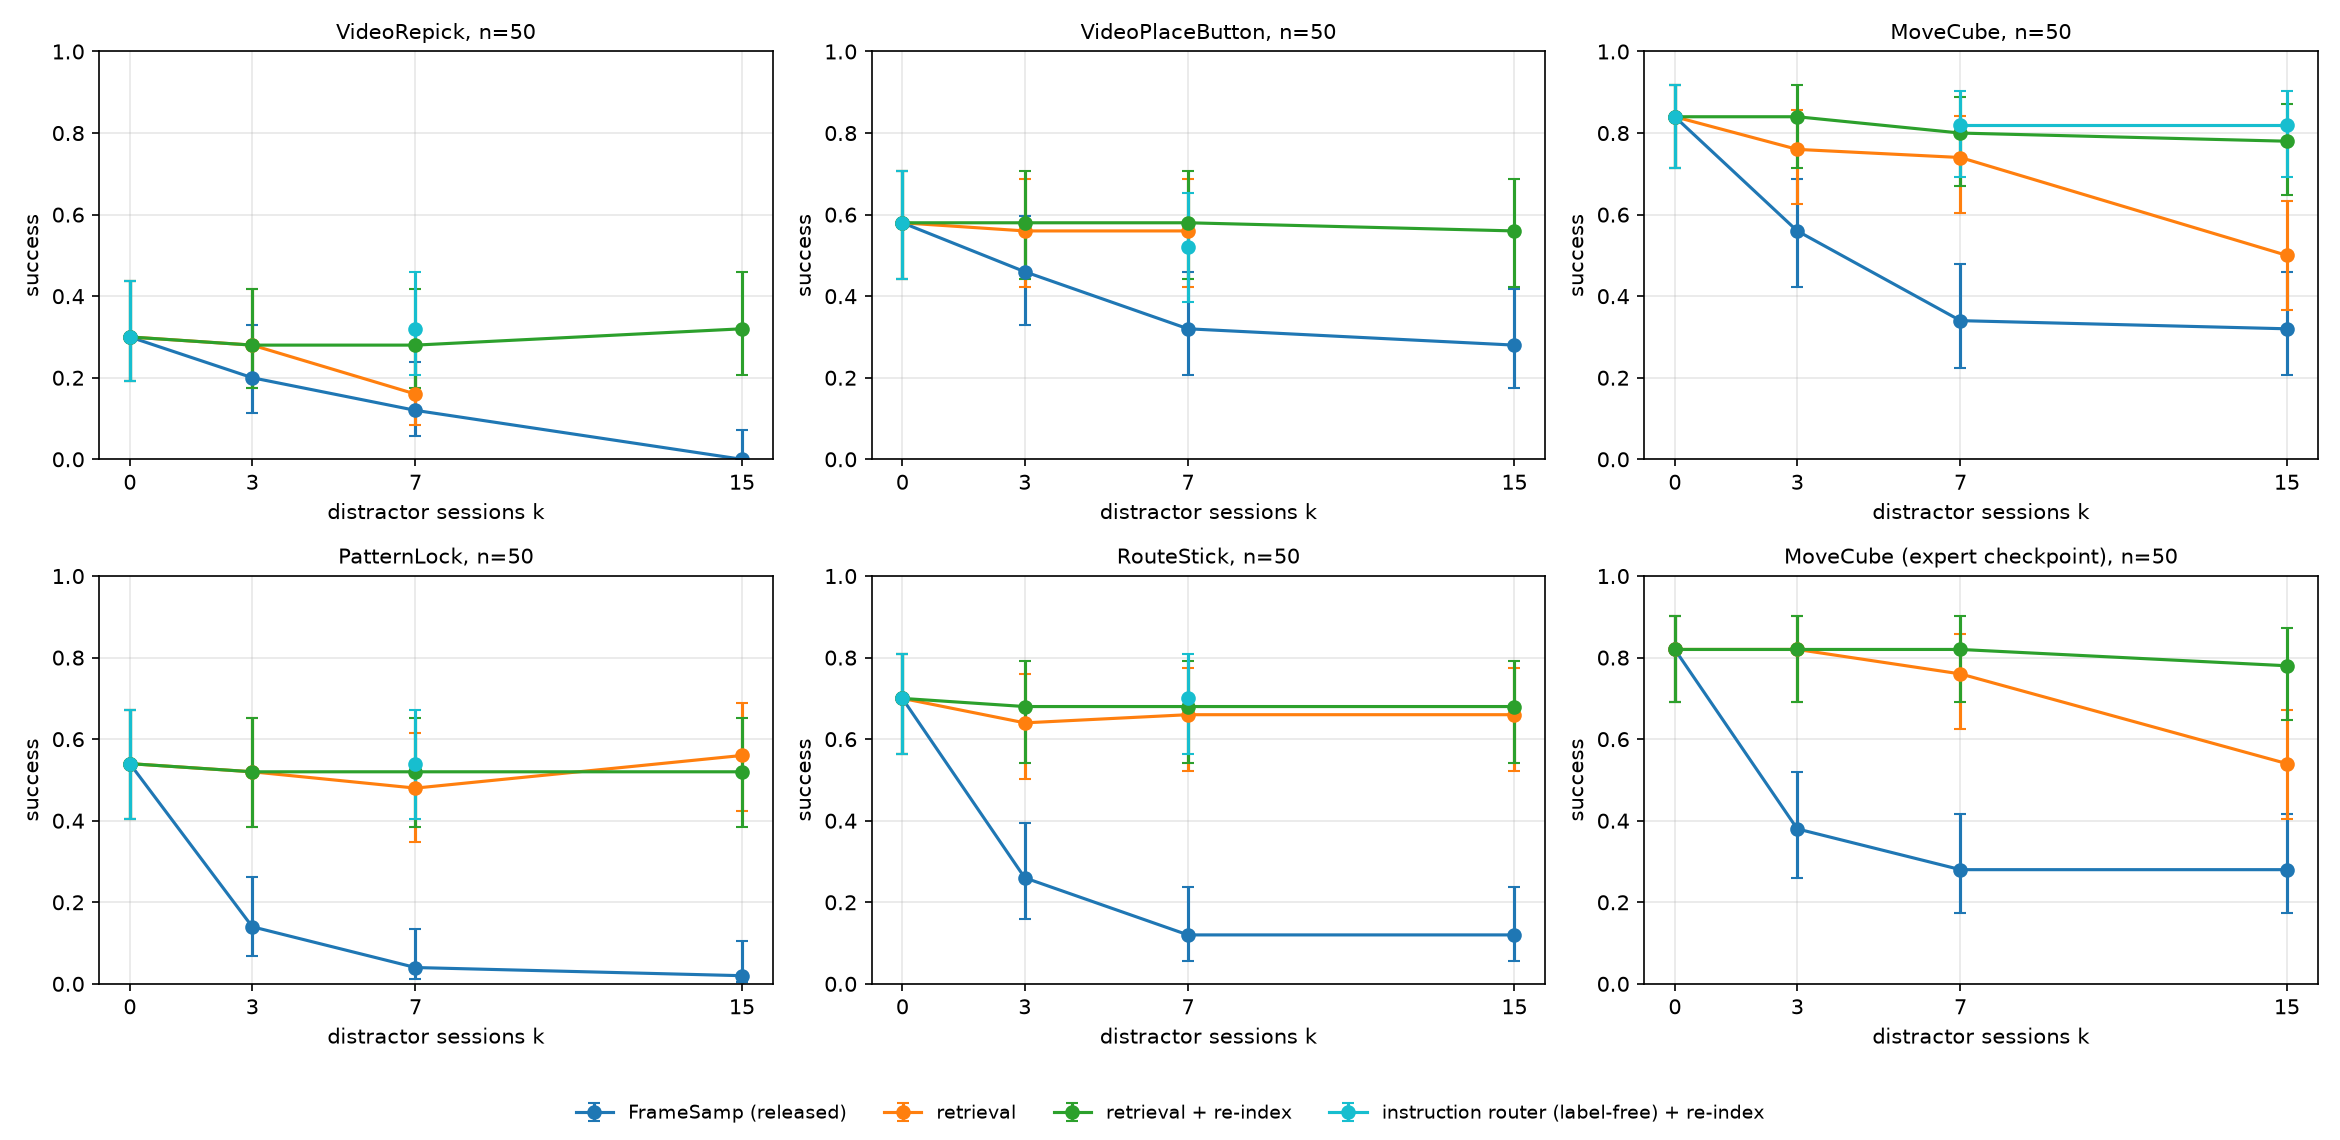
\includegraphics[width=.9\linewidth]{fig/success_vs_k_all.png}
\caption{Standard protocol, success against the number of distractor sessions $k$: released $\pi_{0.5}$ FrameSamp, retrieval, retrieval + re-indexing and the instruction router (Wilson 95\% intervals, $n{=}50$, test split; five tasks with the modulation checkpoint, MoveCube also with the expert checkpoint). The released models collapse; the label-free managers are flat out to $k{=}15$; the gap between the routed curves at large $k$ is the positional shift.}
\label{fig:k}
\end{figure}

\textbf{Same-scene sessions.} For each scene instance we record, after the lesson video, the robot replaying the post-demonstration joint trajectory of a recorded episode of another task for 256 steps from the reset state, and keep 32 evenly spaced front frames and their states. Four such sessions are generated per scene; three are used and inserted at random positions among the four other-task distractors. The scene is reset before the query episode; we verify the reset by comparing the first query frame's fingerprint with the first lesson frame's. Caches exist for the test split of MoveCube, RouteStick, PatternLock and VideoPlaceButton, the val split of RouteStick and MoveCube, and the train split of seven tasks (used for router training and the margin sweep).

\textbf{Label-trained router.} The session router scores each session from attention over its frames' SigLIP features conditioned on the current view, trained with a cross-entropy over sessions. Training examples are built from the train split's lesson videos, other-task distractor units and, for the same-scene routers, the same-scene sessions of 50 training scenes per task. For leave-one-task-out training the held-out task's lesson videos \emph{and} its recorded units are removed from the negative pool; omitting the latter leaks the held-out task into training (a first run with this leak also scored $.44$ on MoveCube, so the conclusion does not depend on it).

\textbf{Instruction router.} HF \texttt{google/siglip-so400m-patch14-384}; a session is represented by up to 32 of its raw front frames; the current view is the latest frame of the current episode. Scene score $=\max_f \cos(e_f, e_{\mathrm{view}})$; gate: score $\ge$ best $-$ margin; instruction score $=\max_f\cos(e_f, e_{\mathrm{text}})$; one decision per episode. A first implementation computed the scene gate on the policy's own pooled features, whose max-over-frames cosines differ by under $.003$ across sessions; that gate admitted every session and the system still scored $.60$ on RouteStick and $.58$ on MoveCube, with a few episodes routed to other-task sessions. We report the SigLIP-gated version.

\begin{figure}[h]
\centering
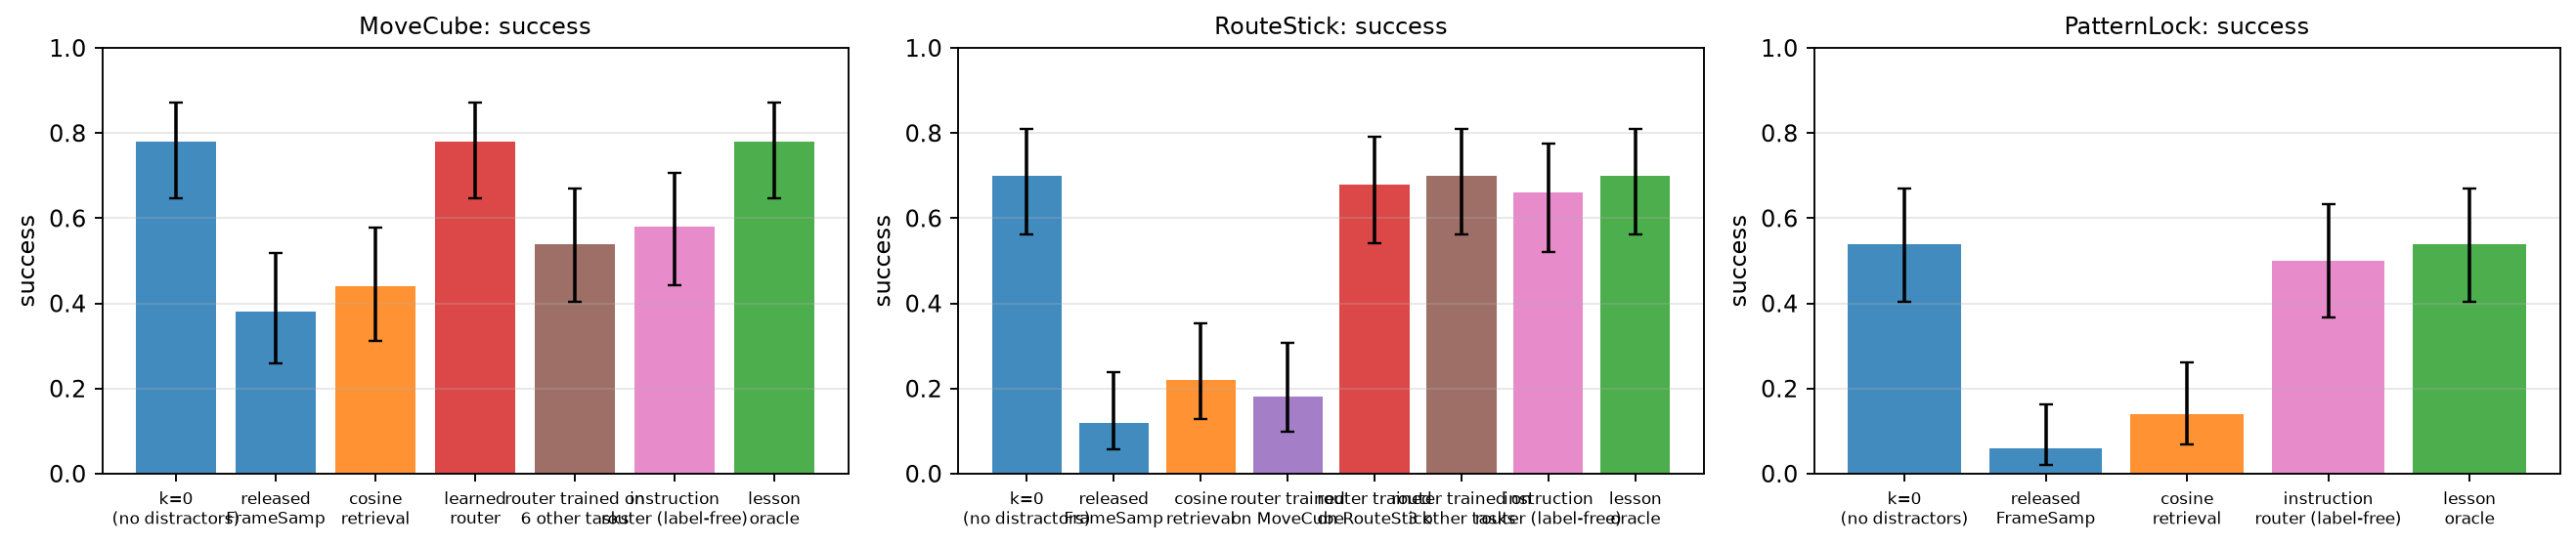
\includegraphics[width=\linewidth]{fig/hard_routing_main.png}
\caption{Hard routing, test split ($n{=}50$; routed systems re-indexed; Wilson 95\% intervals; slot shares in Figure~\ref{fig:hard_app}). Cosine retrieval routes to replays; label-trained routers recover the oracle in-task and transfer in one direction; the label-free instruction router recovers it on RouteStick and PatternLock.}
\label{fig:hard}
\end{figure}

\begin{table}[h]
\centering\small
\caption{Hard condition ($k{=}7$, three same-scene replays, $n{=}50$ per cell): success, episodes the instruction router sent to the lesson, and exact paired McNemar $p$-values on the discordant episodes.}
\label{tab:hardstats}
\setlength{\tabcolsep}{3.5pt}
\resizebox{\linewidth}{!}{\begin{tabular}{llccccc|c|cccc}
\toprule
task & split, ckpt & $k{=}0$ & released & cosine & router & oracle & routed & rel.\ vs $k{=}0$ & cosine vs rel. & router vs rel. & router vs oracle\\
\midrule
MoveCube & test, modul & .78 & .38 & .44 & .58 & .78 & 20/50 & $1\mathrm{e}{-5}$ & .55 & .013 & .006\\
MoveCube & val, modul & .86 & .32 & .30 & .56 & .80 & -- & $2\mathrm{e}{-8}$ & 1.0 & .008 & .002\\
MoveCube & test, expert & .82 & .34 & .44 & .60 & .90 & -- & $8\mathrm{e}{-6}$ & .33 & .007 & $3\mathrm{e}{-4}$\\
RouteStick & test, modul & .70 & .12 & .22 & .66 & .70 & 48/50 & $4\mathrm{e}{-9}$ & .27 & $1\mathrm{e}{-7}$ & .62\\
RouteStick & val, modul & .58 & .14 & .18 & .44 & .56 & -- & $3\mathrm{e}{-6}$ & .79 & $7\mathrm{e}{-4}$ & .03\\
PatternLock & test, modul & .54 & .06 & .14 & .50 & .54 & 46/50 & $8\mathrm{e}{-7}$ & .34 & $3\mathrm{e}{-6}$ & .62\\
VideoPlaceButton & test, modul & .58 & .24 & .52 & .42 & .56 & -- & $8\mathrm{e}{-5}$ & .003 & .02 & .04\\
\bottomrule
\end{tabular}}
\end{table}

\textbf{Gate margin.} With margin $.05$ the router matched the oracle under same-scene distractors but, on the standard protocol, admitted other-task sessions recorded in equally sparse scenes and sometimes chose one (MoveCube $k{=}7$: $.68$ with 35 of 50 decisions to the lesson). We therefore swept the margin offline on the train split only (three seeds $\times$ 50 scenes $\times$ 8 tasks, query $=$ an execution-phase view), Table~\ref{tab:margin}, and fixed $.03$ before any test-split run with it. On the hard condition the choice is immaterial: $.03$ vs $.05$ gives MoveCube $.58/.58$, RouteStick $.66/.66$, PatternLock $.50/.50$ and expert-checkpoint MoveCube $.60/.64$, with the same per-episode outcome in 48 of 50 episodes in the latter two cases.

\begin{table}[h]
\centering\small
\caption{Offline routing accuracy of the instruction router against the gate margin (train split, 8 tasks). ``Standard'': lesson + 4 other-task sessions; ``hard'': lesson + 3 same-scene + 4 other-task sessions.}
\label{tab:margin}
\begin{tabular}{lccccccc}
\toprule
setting & scene only & $.01$ & $.02$ & $.03$ & $.05$ & $.08$ & no gate\\
\midrule
standard & 1.00 & .99 & .99 & .99 & .94 & .80 & .67\\
hard & .09 & .63 & .69 & .69 & .69 & .59 & .50\\
\bottomrule
\end{tabular}
\end{table}

\begin{figure}[h]
\centering
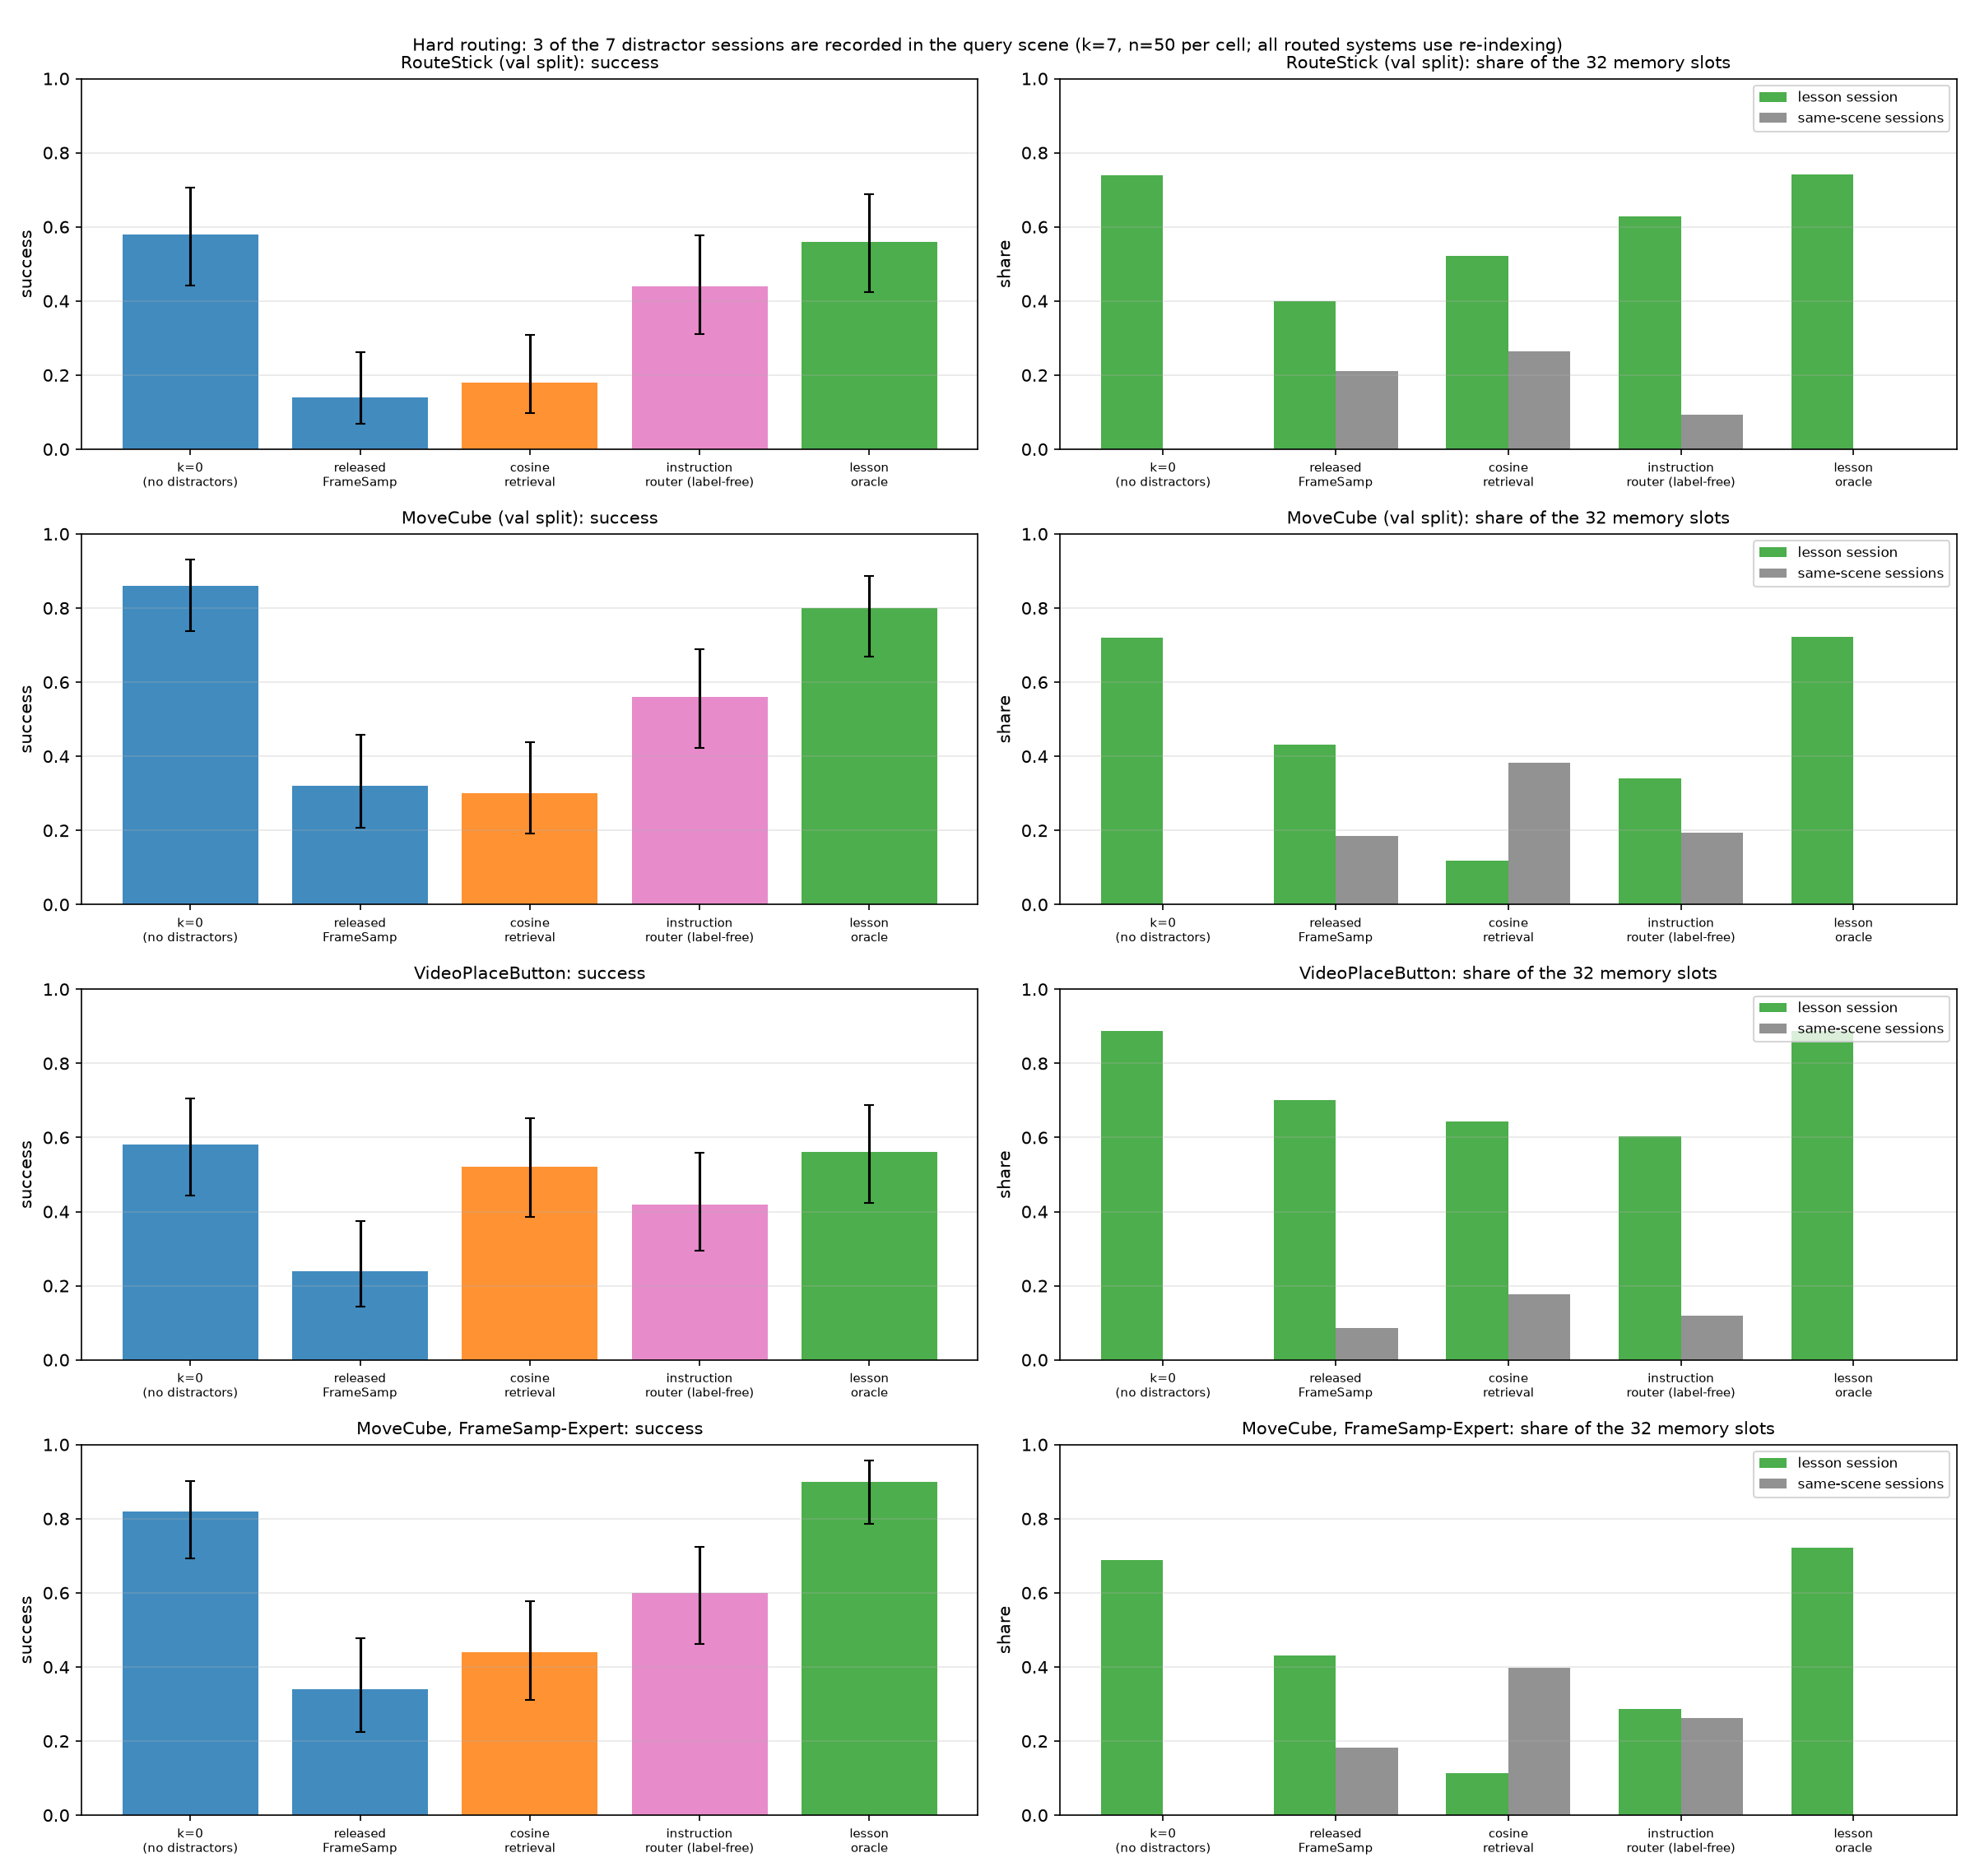
\includegraphics[width=\linewidth]{fig/hard_routing_val.png}
\caption{Hard routing, additional rows ($k{=}7$ with 3 same-scene distractors, $n{=}50$, all routed systems re-indexed; right panels: share of the 32 slots given to the lesson and to same-scene sessions). Rows: RouteStick and MoveCube on the val split, two independent sets of scene instances and same-scene recordings; VideoPlaceButton on the test split, where cosine retrieval survives because the demonstration video is visually set apart from the live scene; MoveCube with the FrameSamp-Expert checkpoint.}
\label{fig:hard_app}
\end{figure}

\section{Fine-tuning study}
\label{app:train}
\textbf{Data.} 100 recorded episodes of each of MoveCube, RouteStick, VideoRepick, VideoPlaceButton and VideoUnmask from the benchmark's datasets (500 episodes, 263{,}049 frames, 112{,}328 execution steps). The policy's SigLIP features (16 tokens per frame) are computed once per frame with the released image encoder, which is frozen throughout, so a training sample is a choice of 32 frame indices and their positions; this makes the three training distributions differ only in the memory they present.
\textbf{Distributions.} \sys{control}: the released recipe, even sampling over the episode's own history, positions $0..t$. \sys{shift}: the same frames, with every execution frame's position moved by $32k$ for $k$ drawn from $\{0,1,3,7,15\}$ ($k{=}0$ with probability $.2$), i.e. the layout produced by a session manager that keeps the lesson at its own positions and the current episode $32k$ steps later. \sys{interf}: the buffer [lesson][$k$ 32-frame units of other-task episodes][episode] sampled evenly with true positions, so the lesson's share of the slots falls with $k$ exactly as at test time.
\textbf{Optimisation.} Released training code and hyper-parameters except as stated: all parameters outside the image encoder (2.89B) trained, EMA $.99$ (the saved parameters), AdamW, learning rate $10^{-5}$ with 100 warm-up steps and cosine decay to $10^{-6}$, batch 32, 4000 steps, one H100 (1.1--1.5 steps/s). Losses: \sys{control} $.0030\to.0007$, \sys{shift} $.0043\to.0009$, \sys{interf} $.0060\to.0010$; the released checkpoint's loss on the interference buffer is thus four times its loss on its own recipe, and the fine-tune removes most of the difference within 400 steps. Checkpoints at 1000 steps gave MoveCube $k{=}7$ $.24$/$.26$ (\sys{control}/\sys{interf}) and retrieval $k{=}15$ $.62$ (\sys{shift}); the 4000-step numbers are in Table~\ref{tab:train}. Val-split replication of the MoveCube retrieval / retrieval + re-index cells at $k{=}15$ ($n{=}50$ new scene instances): released $.54/.74$, \sys{control} $.54/.74$, \sys{shift} $.60/.76$; pooled with the test split, the re-indexing gap is $.24$ (released, $p<.01$), $.13$ (\sys{control}, $p=.08$) and $.10$ (\sys{shift}, $p=.17$). The three runs cost about 20 USD of H100 time; their evaluation about 20 USD of A10G time.

\section{Vision--language verifier}
\label{app:vlm}
Qwen2.5-VL-7B-Instruct, six frames per session as a filmstrip, question ``Does the robot \textit{<instruction>} in these frames?'', score $=$ logit(yes) $-$ logit(no) computed in float32 from the last hidden state (bf16 logits are quantised to ${\sim}.125$ and tie). Offline accuracy of picking the lesson among candidates on 50 training scenes per task: lesson vs 3 same-scene replays, RouteStick $.86$, MoveCube $.68$; lesson vs 4 other-task sessions, $.94$ and $.62$; full 8-way, $.84$ and $.54$. A comparative query (four filmstrips, ``in exactly one the robot \textit{<instruction>}; which?'') was worse ($.44$, $.48$). SigLIP zero-shot on the same offline sets: scene-gated instruction match RouteStick $.86$, MoveCube $.49$ (8-way).

\section{Reproducibility}
Code for the memory manager, the evaluator with the same-scene condition, the routers and their training, the fine-tuning pipeline and the serving app, together with every per-episode result file and the script that reproduces each statistic in this paper, are at \url{https://github.com/hanshaunlee/blame-the-bowl}. All result files hold per-episode rows (system, $k$, episode, success, steps, lesson share, memory-index statistics). Compute for the whole study: about 300 USD, of which the Pantry study is about 40 USD, the fine-tuning study about 45 USD (H100 training and A10G evaluation) and the rest A10G evaluation time.

\end{document}
